\begin{itemize}
    \item L'évolution des technologies du web a conduit à l'avènement de ce qui est communément appelé le Web 2.0.
      La principale caractéristique de ce média est la possibilité aux utilisateur-rices non plus seulement de le consulter, mais aussi d'y contribuer.
    \item Ces nouvelles fonctionnalités ont permis l'apparition d'applications incitant les utilisateur-rices à créer et partager leur propre contenu, ainsi que d'échanger avec d'autres utilisateur-rices à ce sujet.
      \cite{2015-social-media-definition-obar} définit ce type d'applications, \ie les \emph{réseaux sociaux}, de la manière suivante :
      \begin{definition}
        Un réseau social est une application respectant les critères suivants :
        \begin{enumerate}
          \item Elle prend la forme d'une application interactive.
          \item Elle permet à ses utilisateur-rices de produire et de partager leur propre contenu.
            Ce contenu généré par les utilisateur-rices constitue le contenu principal de l'application.
          \item Elle permet à ses utilisateur-rices de possèder et de maintenir leur propre profil sur la plateforme.
          \item Elle encourage ses utilisateur-rices à étendre leur réseau social en se connectant à d'autres utilisateur-rices, voire en créant ou en s'intégrant à des communautés.
        \end{enumerate}
      \end{definition}
      De nos jours, les réseaux sociaux représentent les applications les plus populaires du paysage internet, \eg Facebook compte 2,9 millards d'utilisateur-rices par mois \cite{2022-01-monthly-active-users-social-networks}, Youtube 2,5 milliards \cite{2022-01-monthly-active-users-social-networks}, Wikipedia 788 millions {\cite{2022-09-monthly-active-users-wikipedia}} ou encore Quora 300 millions \cite{2022-01-monthly-active-users-social-networks}.
    \item La démocratisation de ces applications présente plusieurs bienfaits.
      Notamment, nous notons que les réseaux sociaux permettent, en diminuant le coût individuel pour tout à chacun-e de contribuer, d'améliorer la diffusion de l'information \cite{2012-youtube-social-movements-meek,2013-wealth-occupation-networks-theocharis}.
      Aussi, ils contribuent à la création de communautés \cite{2013-understanding-social-media-logic-van-dijck}.
      Finalement, en permettant à chacun-e de partager son savoir, ils permettent la création de bases de connaissances complètes \cite{2005-internet-encyclopaedias-head-to-head,2008-knowledge-sharing-yahoo-answers-adamic}.
    \item Cependant, la conception de réseaux sociaux fait face à de nombreux défis.
      Notamment, ces applications doivent assurer leur haute disponibilité, tolérance aux pannes et capacité de passage à l'échelle en raison de leur popularité et importance dans notre quotidien.
      \begin{definition}[Disponibilité]
          \label{def:availability}
      \end{definition}
      \begin{definition}[Tolérance aux pannes]
      \end{definition}
      \begin{definition}[Capacité de passage à l'échelle]
      \end{definition}
      Pour cela, ces systèmes adoptent une architecture décentralisée\footnotemark, \ie une architecture reposant sur un ensemble de serveurs qui se répartissent la charge de travail et les tâches.
      \footnotetext{Nous utilisons la classification présentée dans \cite{1964-distributed-communications-networks-baran} pour distinguer les architectures systèmes centralisées, décentralisées et distribuées.}
      Malgré ce que le nom de cette architecture peut suggérer, il convient de noter que de manière globale les serveurs jouent toujours un rôle central dans les systèmes décentralisés.
      Par exemple, les serveurs servent à authentifier les utilisateur-rices, à stocker leurs données ou encore à assurer la communication entre utilisateur-rices.
    \item Additionnellement, il convient de préciser que ces serveurs ne sont pas une ressource libre.
      En effet, ils sont mis à disposition et maintenus par la ou les organisations qui proposent le réseau social.
      Ces organisations font alors office d'\emph{autorités centrales} du système, \eg en se portant garantes de l'identité des utilisateur-rices ou encore de l'authenticité d'un contenu.
    \item De part le rôle que jouent les serveurs dans les systèmes décentralisés, ces derniers échouent à assurer un second ensemble de propriétés, que nous jugeons néanmoins fondamentales :
      \begin{definition}[Confidentialité des données]
        \label{def:confidentialite}
      \end{definition}
      \begin{definition}[Souveraineté des données]
        \label{def:souverainete}
      \end{definition}
      \begin{definition}[Pérennité]
        \label{def:perennite}
      \end{definition}
      \begin{definition}[Résistance à la censure]
        \label{def:censorship}
      \end{definition}
      Ainsi, les utilisateur-rices des réseaux sociaux prennent, de manière consciente ou non, le risque que ces propriétés soient transgressées par les autorités auxquelles appartiennent ces applications ou par des tiers avec lesquelles ces autorités interagissent, \eg des gouvernements.
    \item Qui plus est, il convient de noter que les autorités auxquelles appartiennent ces applications, \eg des entreprises, possèdent leurs propres intérêts, \eg leur propre profit.
      De nombreux faits d'actualité ont malheureusement montré que ces autorités ont tendance à privilégier leurs intérêts, quitte à prendre des décisions s'avérant nocives pour une partie de leurs utilisateur-rices.
      Nous pouvons par exemple noter la mise en avant de contenu à caractère raciste \cite{2018-algorithms-oppression-noble}, la non-modération de contenu misogyne \cite{2018-violence-abuse-against-women-amnesty}, l'encouragement à la production de contenu toxique \cite{2021-facebook-files-algorithm-favoring-toxicity-wsj} ou l'inaction et même entrave à la correction des effets délétères de son réseau social sur la santé mentale de ses utilisatrices \cite{2021-facebook-files-instagram-toxic-teen-girls-wsj}.
    \item Ainsi, la présence d'autorités centrales dans les réseaux sociaux représente un danger pour les utilisateur-rices.
      Il nous paraît alors fondamental de proposer des moyens technologiques pour concevoir et déployer des réseaux sociaux alternatifs qui minimisent le rôle des autorités centrales, voire l'éliminent.
    \item Dans cette optique, une piste de recherche que nous jugeons intéressante à étudier est celle présentée dans \cite{localfirstsoftware2019}.
      Dans ce travail, les auteurs proposent un nouveau paradigme de conception d'applications, nommées \acp{LFS}.
      Ce type d'applications se démarque par la place centrale donnée aux utilisateur-rices et leurs propres appareils, les éventuels serveurs étant relegués qu'à de simples rôles de support.
    \item \cite{localfirstsoftware2019} identifie 7 propriétés que doivent satisfaire les applications \acp{LFS}, illustrées dans la \autoref{fig:lfs-properties}.
      \begin{figure}[!ht]
        \centering
        \resizebox{\columnwidth}{!}{
          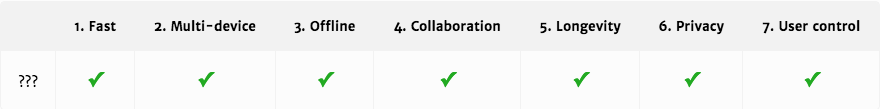
\includegraphics{img/lfs-properties}
        }
        \caption[Caption for lfs-properties]{Liste des propriétés visées par les \acp{LFS}\footnotemark}
        \label{fig:lfs-properties}
      \end{figure}
      \footnotetext{Source : \url{https://www.inkandswitch.com/local-first/\#towards-a-better-future}}
      Ces propriétés se recoupent en grande partie avec celles que nous avons identifiées précédemment :
      \begin{enumerate}
        \item Le fonctionnement en mode hors-ligne et le fonctionnement avec une latence minimale sont tous deux assurés en privilégiant la disponibilité \cite{pacelc2012} (\autoref{def:availability}).
        \item Le respect de la vie privée des utilisateur-rices correspond à la propriété de confidentialité (\autoref{def:confidentialite}).
        \item Le contrôle des utilisateur-rices sur leurs données correspond à la propriété de souveraineté (\autoref{def:souverainete}).
        \item La longétivité de l'application correspond aux propriétés de pérennité (\autoref{def:perennite}) et de résistance à la censure (\autoref{def:censorship}).
      \end{enumerate}
      Notons qu'il découle de ces propriétés que les applications \acp{LFS} sont fondamentalement \ac{P2P}.
    \item De manière similaire, observons que ce paradigme met en lumière une dernière propriété des applications \acp{LFS} :
      \begin{definition}[Collaborative]
        \label{def:collaborative}
        Une application collaborative est une application permettant à plusieurs utilisateur-rices ou robots de travailler ensemble pour réaliser une tâche.
        Dans ce manuscrit, nous considérons qu'une collaboration peut prendre la forme d'une discussion, \eg en participant à un fil de discussion d'une plateforme de questions et réponses, ou d'une édition collaborative d'un contenu, \eg en participant à la rédaction d'une page de wiki.
      \end{definition}
    % \item \mnnote{TODO: Voir si angle écologique/réduction consommation d'énergie peut être pertinent.}
    \item Ainsi, \cite{localfirstsoftware2019} établit un paradigme de conception d'applications correspondant à notre vision.
      Cependant, de nombreuses problématiques de recherche identifiées dans ce travail sont encore non résolues et entravent la démocratisation des applications \acp{LFS}.
    \item Notamment, les applications \acp{LFS} se doivent de répliquer les données entre appareils pour permettre :
      \begin{enumerate}
        \item Le fonctionnement en mode hors-ligne et le fonctionnement avec une faible latence.
        \item Le partage de contenu entre appareils d'un-e même utilisateur-rice.
        \item Le partage de contenu entre utilisateur-rices pour la collaboration.
      \end{enumerate}
    \item Cependant, compte tenu des propriétés visées par les applications \acp{LFS}, plusieurs contraintes restreignent le choix des méthodes de réplication possibles.
      Ainsi, pour permettre le fonctionnement en mode hors-ligne de l'application, \ie la consultation et la modification de contenu, les applications \acp{LFS} doivent relaxer la propriété de cohérence des données.
      \begin{definition}[Cohérence]

      \end{definition}
      Les applications \acp{LFS} ne peuvent donc pas reposer sur des méthodes de réplication dites pessimistes, \ie qui empêchent toutes modifications concurrentes d'une même donnée.
    \item Les applications \acp{LFS} doivent donc adopter des méthodes de réplication dites optimistes \cite{2005-optimistic-replication-saito}.
      Ces méthodes autorisent chaque noeud possédant une copie de la donnée de la consulter et de la modifier sans coordination au préalable avec les autres noeuds.
      L'état des copies des noeuds peut donc diverger temporairement.
      Un mécanisme de synchronisation permet ensuite aux noeuds de partager les modifications effectuées et de les intégrer de façon à converger à terme \cite{10.1145/224057.224070}, \ie obtenir à terme de nouveau des états équivalents.
    \item Cependant, il convient de noter que les méthodes de réplication optimistes autorisent la génération en concurrence de modifications provoquant un conflit, \eg la modification et la suppression d'une même page dans un wiki.
      Un mécanisme de résolution de conflits est alors nécessaire pour assurer la convergence à terme des noeuds.
    \item De nouveau, le modèle du système des applications \acp{LFS} limitent les choix possibles concernant les mécanismes de résolution de conflits.
      Notamment, les applications \acp{LFS} ne disposent d'aucun contrôle sur le nombre de noeuds qui compose le système, \ie le nombre d'appareils utilisés par l'ensemble de leurs utilisateur-rices.
      Le nombre de noeuds peut donc croître de manière non-bornée.
      La complexité algorithmique des mécanismes de résolution de conflits doit donc être indépendante de ce paramètre, ou alors en être fonction uniquement de manière logarithmique.
    \item De plus, ces noeuds n'offrent aucune garantie sur leur stabilité.
      Des noeuds peuvent donc rejoindre et participer au système, mais uniquement de manière éphèmère.
      Ce phénonème est connu sous le nom de \emph{churn} \cite{understandingChurnP2PNetworks2006}.
      Ainsi, de part l'absence de garantie sur le nombre de noeuds connectés de manière stable, les applications \acp{LFS} ne peuvent pas utiliser des mécanismes de résolution de conflits reposant sur une coordination synchrone d'une proportion des noeuds du système, \ie sur des algorithmes de consensus \cite{1998-paxos-lamport, 2014-raft-ongaro}.
    \item Ainsi, pour permettre la conception d'applications \acp{LFS}, il convient de disposer de mécanismes de résolution de conflits pour l'ensemble des types de données avec une complexité algorithmique efficace par rapport au nombre de noeuds et ne nécessitant pas de coordination synchrone entre une proportion des noeuds du système.
\end{itemize}

% \subsection{Réplication de données mutables}

% Les techniques de réplication de données mutables introduisent de la redondance de données dans les systèmes.
% Cette redondance a pour but et effet d'améliorer plusieurs propriétés des systèmes :

% \begin{definition}[Disponibilité]
% \end{definition}

% \begin{definition}[Tolérance aux pannes]
% \end{definition}

% \begin{definition}[Capacité de passage à l'échelle]
% \end{definition}

% \begin{definition}[Latence]
% \end{definition}

% Les techniques de réplication de données peuvent être classées en deux approches : les \emph{techniques de réplication de données pessimistes} et les \emph{techniques de réplication de données optimistes}.
% Ces deux catégories offrent des compromis différents vis-à-vis des propriétés décrites par les théorèmes CAP \cite{brewer_2000_podc} et PACELC \cite{pacelc2012}.
% Notamment, la différence entre ces catégories concerne le cas de la propriété de \emph{cohérence}.

% \begin{definition}[Cohérence]
% \end{definition}

% \subsection{Réplication de données pessimiste}

% Les techniques de réplication de données dites \emph{pessimistes} privilègie la cohérence des données.
% Notamment, ces techniques empêchent les modifications en concurrence d'une même donnée.
% Pour cela, plusieurs approches sont possibles.

% \begin{itemize}
%     \item Première approche consiste à utiliser un verrou.
%     \item Seconde approche consiste à utiliser un système de vote pour décider de la prochaine modification.
%         Consensus, élection de leader, SMR.
%     \item Le choix de privilégier la cohérence des données se fait au détriment de la disponibilité, tolérance aux pannes, capacité de passage à l'échelle et latence.
%         Par exemple, un système basé sur un leader deviendra temporairement indisponible lors d'une panne de son leader, le temps que la panne soit détectée et qu'un nouveau leader soit élu.
% \end{itemize}

% \subsection{Réplication de données optimiste}

% À l'inverse, les techniques de réplication de données dites \emph{optimistes} jugent acceptable de relâcher les contraintes existantes sur la cohérence des données.
% Dans ce paradigme, chaque noeud qui possède une copie de la donnée répliquée peut la consulter et la modifier à tout moment, sans coordination préalable avec les autres noeuds.
% Les copies des noeuds sont donc autorisées à diverger de manière temporaire.

% Les modifications effectuées par chacun sont ensuite diffusées pour être intégrées par l'ensemble des noeuds et converger de nouveau, \ie atteindre des états équivalents.
% Cependant, certaines modifications effectuées en concurrence par les noeuds peuvent provoquer des conflits.
% \mnnote{NOTE: Pourrait insérer exemple de conflits de l'édition collaborative ici.}
% Des mécanismes de résolution de conflits, potentiellement automatiques, sont alors requis pour assurer la convergence à terme.

% Cette approche permet donc de privilégier la disponibilité, tolérance aux pannes, capacité de passage à l'échelle et latence en échange de la cohérence forte.

% Dans le cadre de cette thèse, nous nous intéressons aux techniques de réplication de données optimistes.
